\section{Metod of manufactured solutions}
Method of manufactured solutions (MMS) was used to verify the implementation.
We use a manufactured solution for $h(x,t)$ and $u(x,t)$.
Choose a simple sine wave function for the water height $h$ and a corresponding $u$ that satisfies the shallow water equations.
Consider
\begin{align*}
    h(x,t) &= h_0 + A \cos(\omega t - kx), \\
    u(x,t) &= \frac{ A \omega }{k h_0}  \cos(\omega t - kx),
\end{align*} 
where $h_0$ is the constant base depth, $A$ is the amplitude of the wave, $k$ is the wave number, and $\omega$ is the angular frequency.

We begin by computing the source terms $S_h$ and $S_u$.
First we compute the partial derivatives
\begin{align*}
    h_t &= ,\\
    u_t &=  \\
\end{align*}
which gives (using the chain rule)
\begin{align*}
    {(hu)}_x &= h_x u + h u_x \\
    &= 
\end{align*}



\begin{figure}[htbp]
    \centering
    % First row
    \begin{subfigure}[b]{0.4\textwidth}
        \centering
        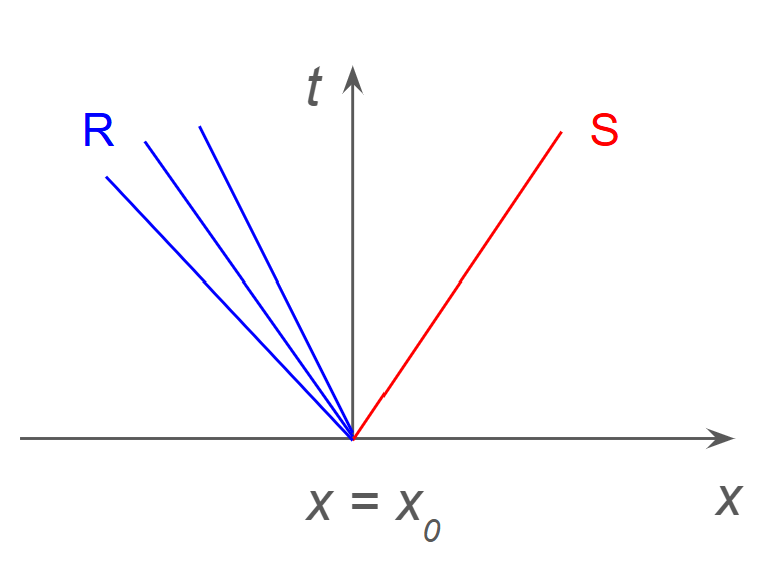
\includegraphics[width=\textwidth]{C:/Users/Matteo/Shallow-Water-Equations/figs/waves-LRRS.png}
        \caption{Left rarefaction wave, right shock wave.}\label{fig:waves-LRRS}
    \end{subfigure}
    \hspace{0.02\textwidth} % Small horizontal space between figures
    \begin{subfigure}[b]{0.4\textwidth}
        \centering
        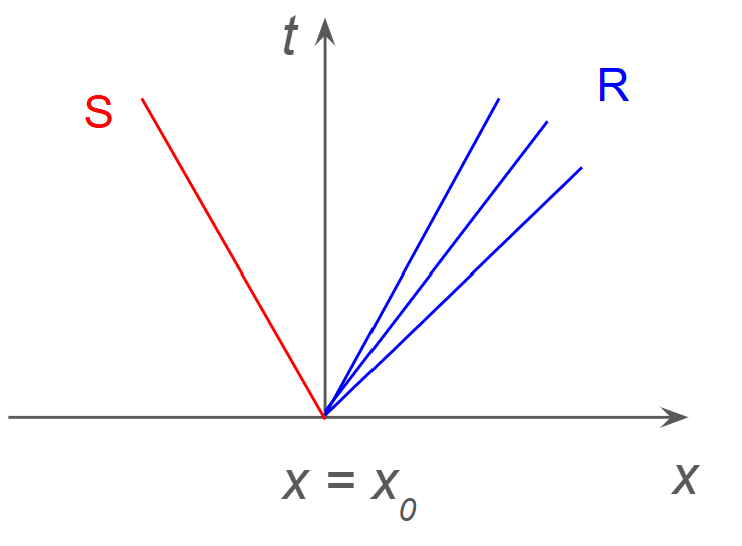
\includegraphics[width=\textwidth]{C:/Users/Matteo/Shallow-Water-Equations/figs/waves-LSRR.png}
        \caption{Left shock wave, right rarefaction wave.}\label{fig:waves-LSRR}
    \end{subfigure}
    
    % Second row
    \begin{subfigure}[b]{0.4\textwidth}
        \centering
        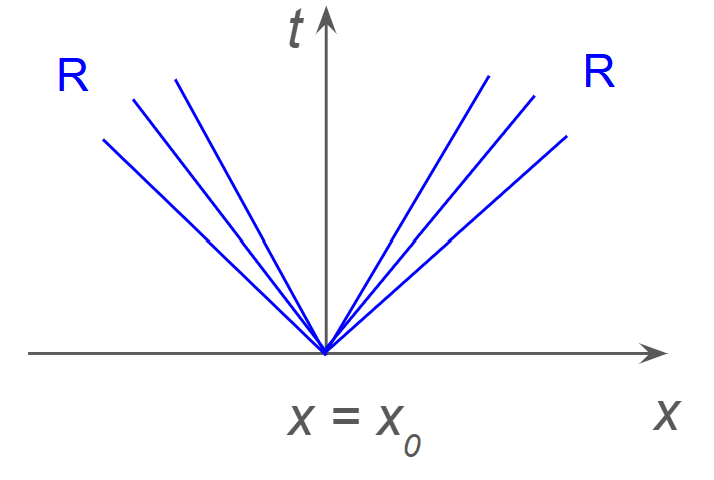
\includegraphics[width=\textwidth]{C:/Users/Matteo/Shallow-Water-Equations/figs/waves-LRRR.png}
        \caption{Left and right rarefaction waves.}\label{fig:waves-LRRR}
    \end{subfigure}
    \hspace{0.02\textwidth} % Small horizontal space between figures
    \begin{subfigure}[b]{0.4\textwidth}
        \centering
        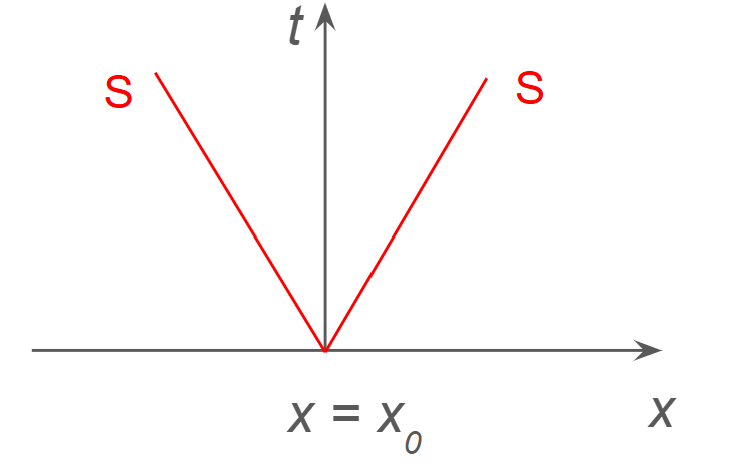
\includegraphics[width=\textwidth]{C:/Users/Matteo/Shallow-Water-Equations/figs/waves-LSRS.png}
        \caption{Left and right shock waves.}\label{fig:waves-LSRS}
    \end{subfigure}
    \caption{Four possible wave patterns in the solution of the Riemann problem.}\label{fig:wave-patterns}
\end{figure}

